%************************************************
\chapter{Causal Hypotheses}
\label{chapter:causal_hypotheses}
%************************************************

\section{Representing Static Space}

Spatial arrangements of static symbols are created by the reflective
thinking layers.  Static symbols are not contained within the physical
layer, but these symbols are used to represent transitions from the
past to the future, which are in turn used to create relationships
between causes and effects that are used for planning.  Thinking
activities use these Spatial arrangements of symbols to think about
the given activities of the physical layer as well as planning in the
first-order reflective layer.

\section{Representing Simultaneities and Transitions}

As {\mbox{\autoref{equation:define_symbol_referent_graph}}} states,
each reflective thinking layer can create static symbolic references
to activities in the layers below as well as any static symbolic
activities in or below that layer.  Simultaneities and transitions are
the basis for representing concurrent and sequential event knowledge.
It is a type of static Spatial arrangement between static symbolic
references.  Simultaneities and transitions can be arranged into
sequences back in time, forward in time, as well as organizing time
into binary trees for efficient recall.
\begin{figure}
\center
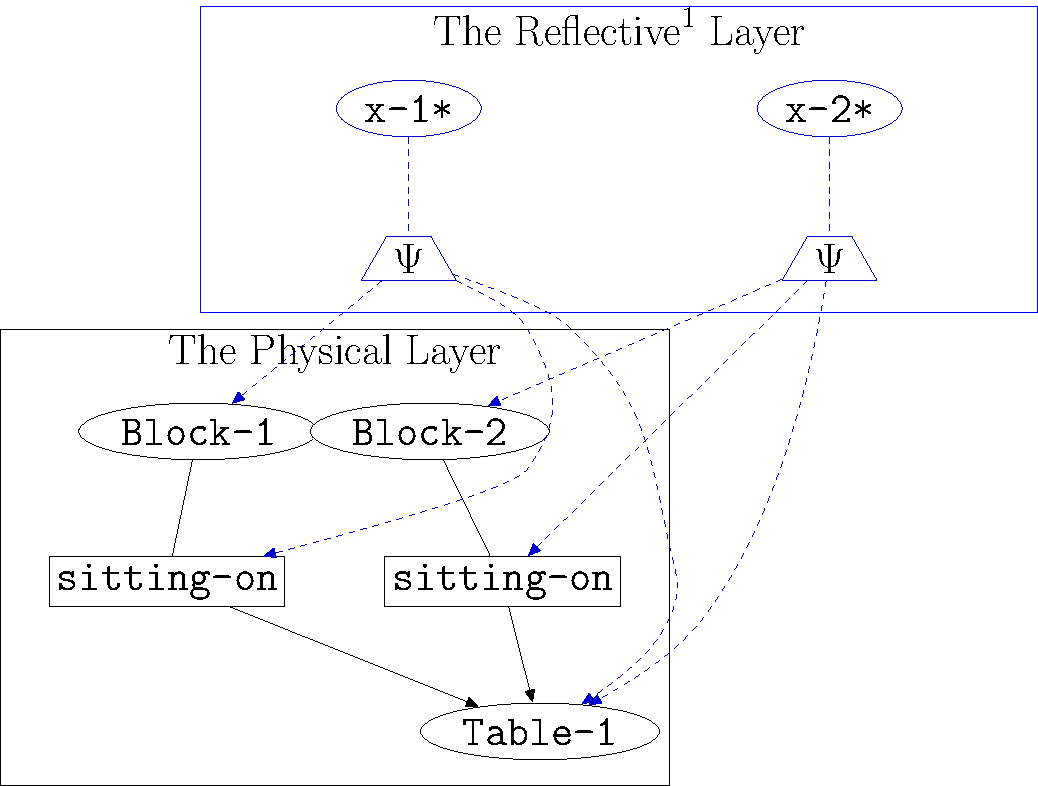
\includegraphics[width=10cm]{gfx/two_example_grounded_symbolic_references}
\caption[Two example symbolic references.]{Two example grounded symbolic references, $x_1^*$ and $x_2^*$.}
\label{figure:two_example_grounded_symbolic_references}
\end{figure}
\begin{figure}
\center
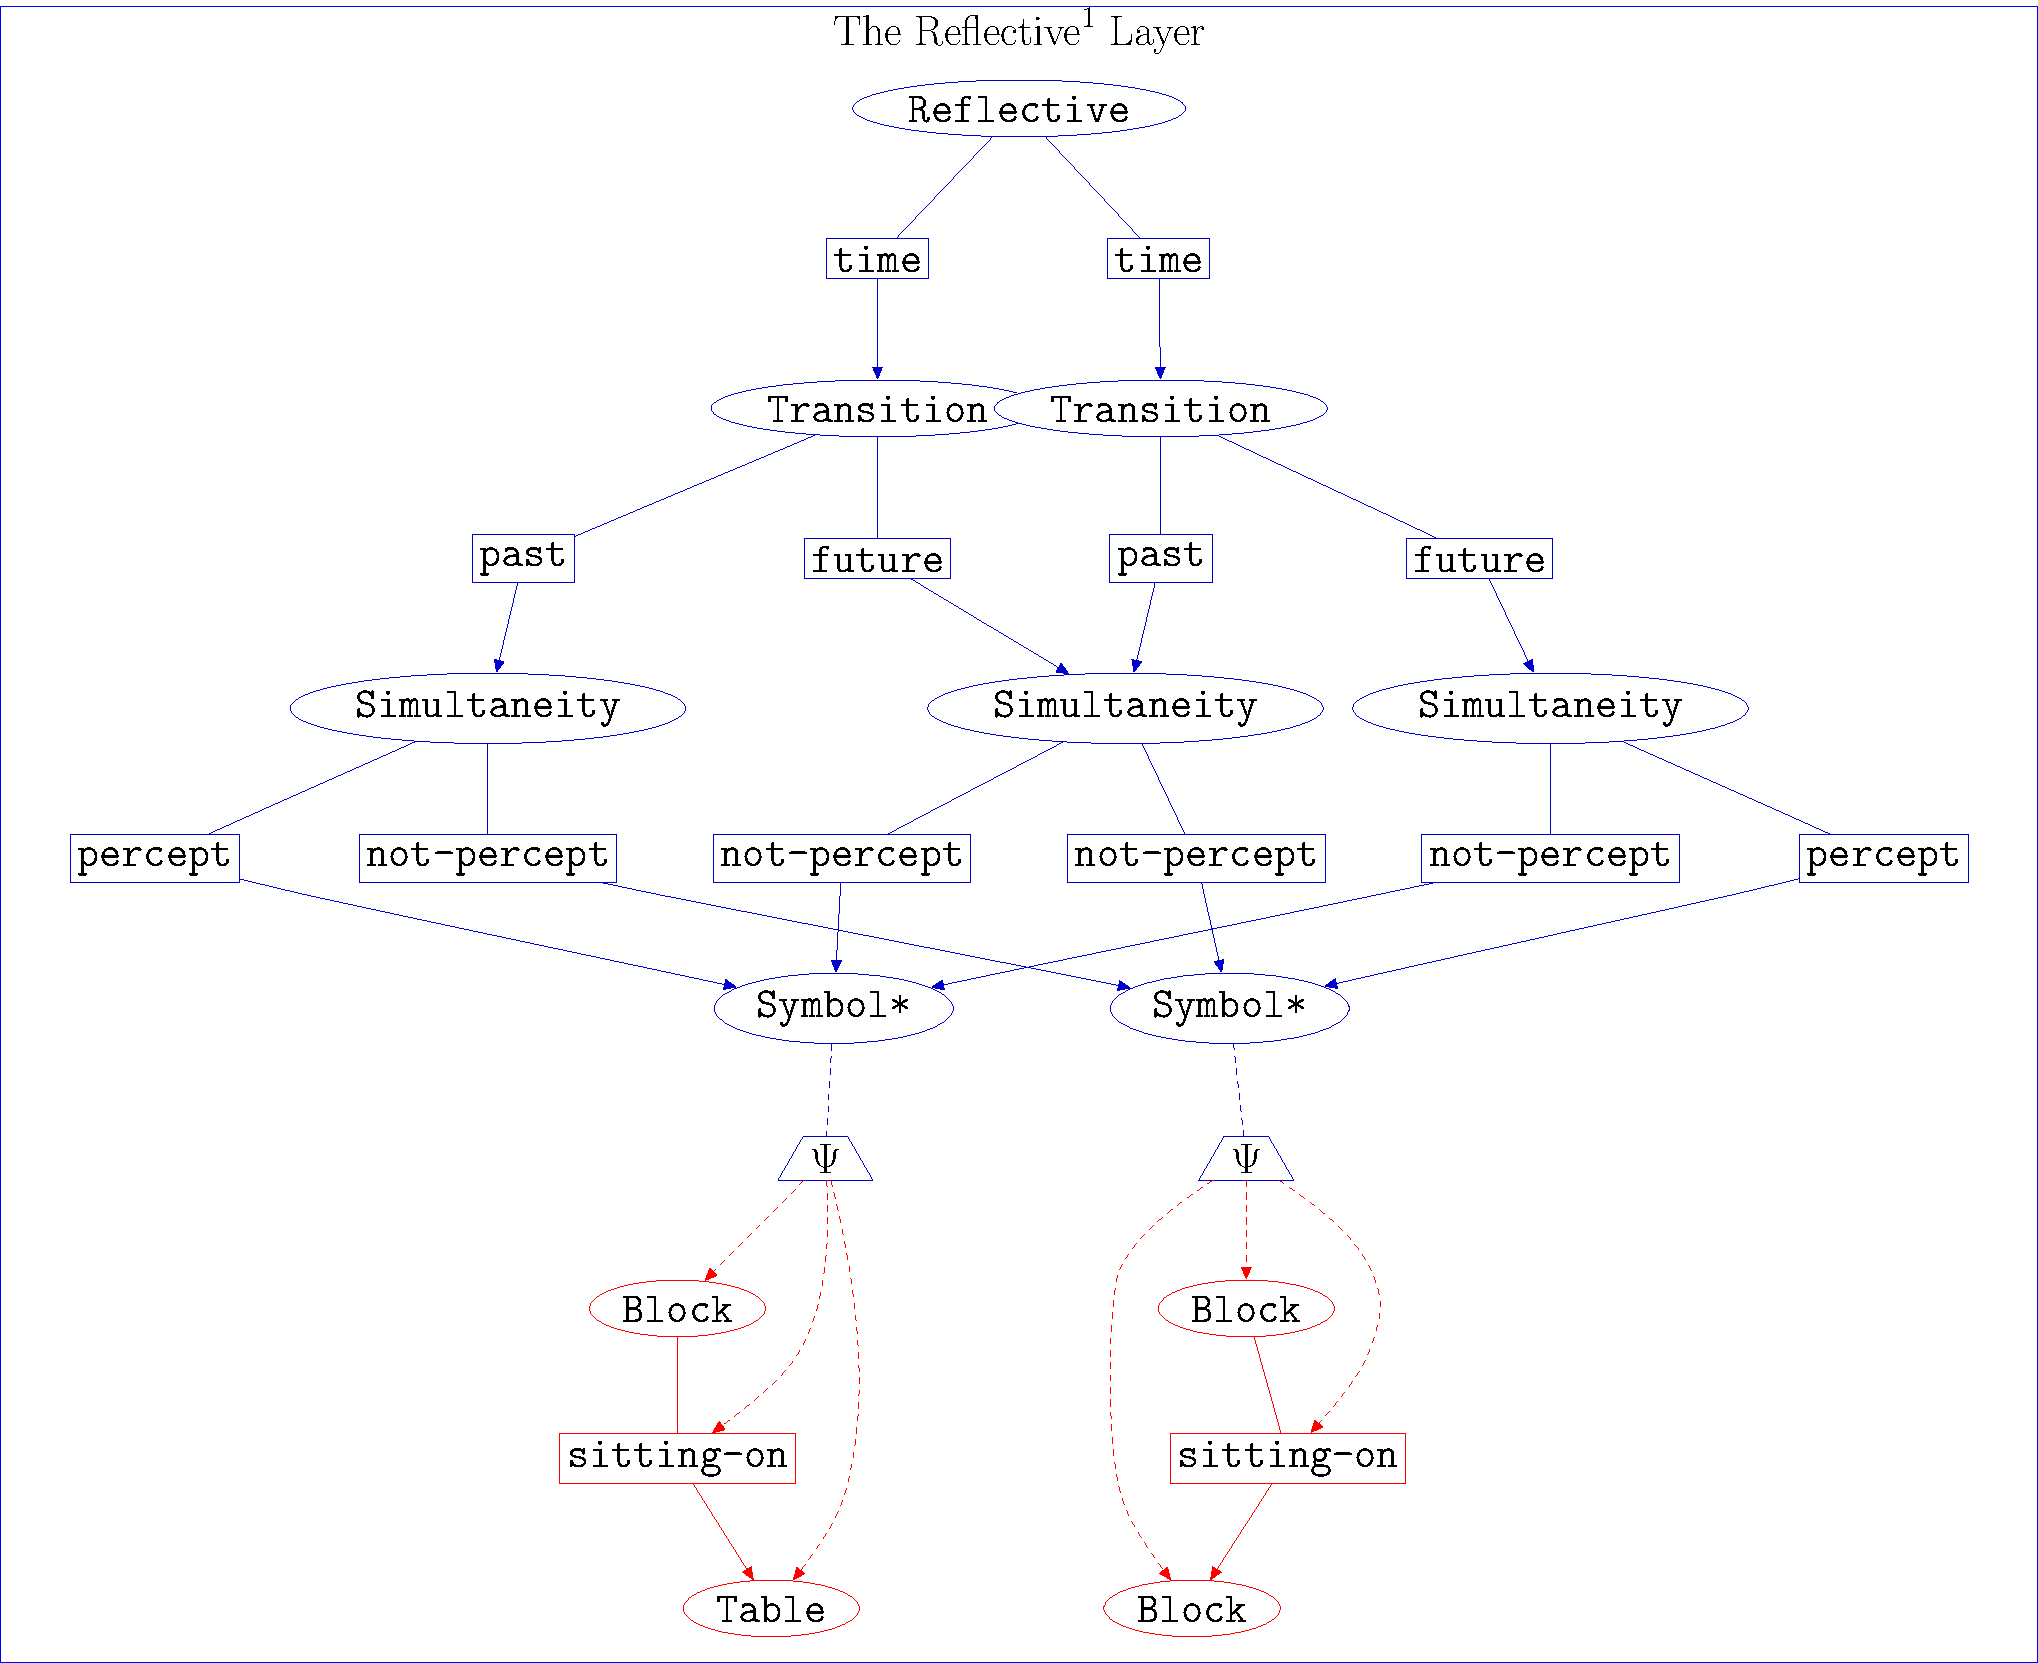
\includegraphics[width=10cm]{gfx/example_transition}
\caption[An example of a transition between simultaneities.]{An
  example of a transition between simultaneities of first-order static
  symbolic references, $x_1^*$ and $x_2^*$.}
\label{figure:example_transition}
\end{figure}










\section{leftovers...}

\section{Simulation States}

At any given point in the simulation, the state, $S$, is static, but
the simulation can have different static states at different time
steps, $n$, giving a number of static states, $S[n]$.  The simulation
process is a discrete stepwise activity.  The simulation step is the
dynamic activity that is not part of the state, $S$, of the simulation
model.  I will now describe a notation for referring to the different
states that result from a simulation process.

Equations~\ref{equation:simulate_first}
and~\ref{equation:simulate_last} show a notation for referring to the
state of a simulation after a number of simulation steps, $n$.
\begin{align}
\label{equation:simulate_first}
S[0] &= \text{\emph{The Initial State}} \\
\label{equation:simulate_last}
S[n] &= \text{\emph{simulate}}~S[n-1]
\end{align}
Equation~\ref{equation:simulate_first} defines $S[0]$ to be
the initial representation of the activities in Duration that are
being simulated; an example of the initial state was given previously
in Equation~\ref{equation:example_initial_state}.
Equation~\ref{equation:simulate_last} introduces an explicit reference
to the activity of simulation with the symbol ``simulate.''  Because I
have not yet defined this activity, these equations still have a
reference to the actual dynamic activity of simulation.  I use this
notation to discuss how the state, $S$, changes during the
actual process of simulation.  I will use the notation in
Equation~\ref{equation:simulate_n_steps} to refer to the state of the
simulation after $n$ actual steps of simulation activity:
\begin{equation}
\label{equation:simulate_n_steps}
S[n] = \text{\emph{simulate}}^n~S[0]
\end{equation}
